\documentclass[a4paper]{article}
\usepackage[T1]{fontenc}
\usepackage[utf8]{inputenc}
\usepackage[polish]{babel}
\usepackage{biblatex}
\usepackage{amsmath, amsfonts}
\usepackage{indentfirst}
\usepackage{graphicx}
\usepackage[nofoot,hdivide={1cm,*,1cm},vdivide={1cm,*,1cm}]{geometry}
\frenchspacing

% dane autora
\author{Franciszek Zdobylak \\ \small{nr ind. 310313}}
\title{\LARGE{Sprawozdanie} \\ \normalsize{Interpolacja metodą Lagrange'a i Newtona}}
\date{\today}

\begin{document}
\maketitle
\abstract
W sprawozdaniu przedstawię metodę interpolacyjną Lagrange'a.
Porównam metodę Lagrange'a z metodą Newtona oraz pokażę sposób zamiany postaci
Lagrange'a na postać Newtona i sprawdzę efektywność tej zamiany.

\section{Różne oblicza postaci Lagrange'a}

Funkcję $f(x)$ interpolujemy w $n+1$ punktach $x_0, x_1, ..., x_n$. Oznaczmy $f_i = f(x_i)$
Postać Lagrange'a wielomianu interpolacyjnego jaką możemy najczęściej spotkać
wygląda tak[1]:
$$ L(x) = \sum_{i=0}^{n} f_i l_i(x) 
\text{\hspace{0.5cm}, gdzie } 
l_i(x) = \prod_{j=0,j\neq i}^n \frac{x - x_j}{x_i - x_j}$$

Widać w niej, że wielomian $ l_i(x) $ przyjmuje wartość $ 1 $ dla $ x = x_i $
oraz wartość $ 0 $ dla $ x_j \neq x_i $. Do obliczeń numerycznych lepiej
wykorzystać lekko zminioną postać:

$$ L(x) = \sum_{i=0}^n w_if_i \prod_{j=0, j \neq i} ^n (x - x_j) 
\text{\hspace{1cm}, gdzie } w_i = \frac{1}{\displaystyle\prod_{j=0, j\neq i}^{n}(x_j - x_i)}$$

Współczynniki $w_i$ nie zależą od punktu $x$, w którym liczymy wartość funkcji, więc można je 
wyliczyć podczas konstruowania wielomianu, dzięki czemu nie trzeba wykonywać
dodatkowych mnożeń podczas wyliczania wartości wielomianu. Do ich wyliczenia można zastosować 
poniższy algorytm \cite{1}. (Działa on w czasie $O(n^2)$ gdzie $n$ to liczba wspóczynników 
do policzenia, czyli liczba wązłów interpolacyjnych.)

\begin{align*}
    a_0^{(0)} &= 1, a_k^{(0)} = 0, \qquad k = 1,...,n
\end{align*}
\begin{align*}
    \left. \begin{array}{l}
    a_k^{(i)} = a_k^{(i - 1)} / (t_k - t_i)\\
    a_i^{(k+1)} = a_i^{(k)} - a_k^{(i)}
  \end{array} 
  \right\} \qquad i = 1,2,...,n,\quad k = 0,1,...,i-1
\end{align*}
\begin{align*}
    w_i  &= a_i^{(n)}, \qquad i = 0,1,...,n
\end{align*}

Warto również zauważyć, że w przypadku gdy interpolujemy wielomian w węzłach równoodległych lub Czebyszewa
postać współczynników znacząco sie upraszcza i możemy je policzyć w czasie liniowym ze wzorów \cite{2} :

\[
  \begin{minipage}{.35\linewidth}
    \centering
    W przypadku węzłów równoodległych:
    $$ w_i = (-1)^i\binom{n}{i}$$
  \end{minipage}
  \begin{minipage}{.35\linewidth}
    \centering
    W przypadku węzłów Czebyszewa:
    $$ w_i = (-1)^i\sin{\frac{(2i+1)\pi}{2n+2}}$$
  \end{minipage}
\]

Mimo iż w trakcie konstruowania wielomianu obliczamy współczynniki $w_i$, to dalej wartość wielomianu
jest liczona w czasie kwadratowym. Chcielibyśmy znaleźć sposób, który pozwoli nam to robić szybciej.
Z pomocą przychodzi postać barycentryczna wielomianu Lagrange'a. Przedstawię krótkie jej wyprowadzenie.

Niech $$l(x) = (x - x_0) \cdots (x - x_n)$$ 
Wtedy $$l_i(x) = l(x)\frac{w_i}{x-x_i}$$
W takim razie:
$$ L(x) = \sum_{i=0}^{n}f_il_i(x) = \sum_{i=0}^nf_il(x)\frac{w_i}{x-x_i} = 
          l(x)\sum_{i=0}^n\frac{w_i}{x-x_i}f_i $$
Zauważmy, że 
$$ 1 = \sum_{i=0}^nL_i(x) = \sum_{i=0}^n\frac{l(x)w_i}{x-x_i} = l(x)\sum_{i=0}^n\frac{w_i}{x-x_i}$$

Więc
$$  L(x) = \frac{L(x)}{1} = 
\frac{l\displaystyle(x)\sum_{i=0}^n\frac{w_i}{x-x_i}f_i}{l\displaystyle(x)\sum_{i=0}^n\frac{w_i}{x-x_i}} = 
\frac{\displaystyle\sum_{i=0}^n\frac{w_i}{x-x_i}f_i}{\displaystyle\sum_{i=0}^n\frac{w_i}{x-x_i}}$$

W takim razie wzór na postać barycentryczną Lagragne'a wygląda w ten sposób:
$$ L(x) = 
          \begin{cases}
            \frac{\displaystyle\sum_{i=0}^n \frac{w_i}{x - x_i}f_i}{\displaystyle\sum_{i=0}^n \frac{w_i}{x - x_i}} & \text{, gdy } x \neq x_k \\
              f_k & \text{, gdy } x = x_k
          \end{cases}
        $$
Do wyliczenia wartości wielomianu używając tej postaci potrzebujemy wykonać 
$2n+3$ operacji mnożenia i $3n+1$ operacji dodawania. (Podczas obliczania 
w postaci Newtona wykonamy $n$ operacji mnożenia i $2n$ dodawania.)


\section{Trochę o postaci Newtona}
Inną postacią wielomianu interpolacyjnego jest postać Newtona. Przedstawia ona się
w ten sposób:
$$ N(x) = \sum_{i=0}^n a_i \prod_{j = 0}^{i-1}(x - x_j) \text{\hspace{1cm}, gdzie }
a_i = f[x_0, x_1, ..., x_i]$$
wyrażenie $ f[x_0, ..., x_k] $ nazywane jest ilorazem różnicowym oraz przedstawia 
się wzorem:
$$ f[x_0, x_1, ..., x_k] = \frac{f[x_0, ..., x_{k-1}] - f[x_1, ..., x_k]}{x_0 - x_k}$$

Do obliczenia współczynników $a_k$ można użyć następującego algorytmu. Jego złożoność jest $O(n^2)$,
gdzie $n$ to liczba współczynników do policzenia(liczba węzłów interpolacyjnych).

\begin{verbatim}
Dla i = 0,..,n:
  a[i] = f(x[i])

Dla i = 1,...n:
  Dla k = i,i+1,...,n:
    a[k] = (a[k] - a[k-1]) / (x[k] - x[k-1])
\end{verbatim}

\section{Błąd interpolacji}
W zadaniu na temat interpolacji warto również wspomnieć o błędzie interpolacji. Błąd interpolacji
dla wielomianu n-tego stopnia wyraża się wzorem:

\begin{align*}
  E_n = \max_{-1\le x\le 1} |f(x) - L_n(x)| &\le \frac{M_{n+1}P_{n+1}}{(n+1)!}\\
  M_{n+1} &= \max_{-1 \le x \le 1} |f^{(n+1)}(x)| \\
P_{n+1} &= \max_{-1 \le x \le 1} |p_{n+1}(x)|, \\
\quad \text{gdzie } p_{n+1}(x) &= (x - x_0)\cdots(x-x_n)
\end{align*}

Można zauważyć, że aby zmniejszyć błąd dla ustalonej funkcji możemy jedynie zmieniać rozłożenie
węzłów interpolacji. Zostało udownione, że najlepszym rozkładem węzłów interpolacji są zera 
wielmianu Czebyszewa. Wtedy wielomian $p_{n+1}(x)$ wyraża się wzorem:
$$ p_{n+1}(x) = 2^{-n}T_{n+1}(x), \quad \text{gdzie $T_{n+1}$ to wielomian Czebyszewa} $$
A błąd interpolacji wynosi:
$$
E_n = \frac{M_{n+1}}{2^n(n+1)!}
$$



\section{Zamiana postaci Lagrange'a na postać Newtona}
Postać Lagrange'a oraz Newtona opisują dokładnie ten sam wielomian, więc 
chcemy, mając wyliczoną postać Lagrange'a, umieć wyliczyć postać Newtona, bez
konstruowania go od nowa.

Od teraz będziemy prezentować postać Lagrange'a w ten sposób:
$$ L(x) = \sum_{i=0}^{n} \sigma_i \prod_{j=0, j\neq i}^{n}(x - x_j) 
\text{\hspace{0.5cm}, gdzie } \sigma_i = w_if_i  = \prod_{j = 0 j\neq i}^n \frac{f_i}{x_i - x_j}$$

Współczynnik $a_k$ w postaci Newtona będzie wyglądał następująco:
$$ a_k = f[x_0, ..., x_k] = \sum_{i=0}^k\frac{f_i}{\displaystyle\prod_{j=0 j \neq i}^k(x_i - x_j)} = 
\sum_{i=0}^{k}\sigma_i \prod_{j=k+1}^{n}(x_i - x_j)$$

Algorytm wyliczania tych współczynników realizuje eliminację Gaussa na równaniu:

$$
\begin{pmatrix}
  a_0 \\ a_1 \\ a_2 \\ \vdots \\ a_n
\end{pmatrix} = 
\begin{pmatrix} \displaystyle
  \displaystyle\prod_{j=1}^n(x_0 - x_j) & 0 & 0 & \cdots & 0 \\
  \displaystyle\prod_{j=2}^n(x_0 - x_j) & \displaystyle\prod_{j=2}^n(x_1 - x_j) & 0 & \cdots & 0\\
  \displaystyle\prod_{j=3}^n(x_0 - x_j) & \displaystyle\prod_{j=3}^n(x_1 - x_j) & \displaystyle\prod_{j=3}^n(x_2 - x_j) & \cdots & 0\\
  \vdots & \vdots & \vdots & & \vdots \\
  (x_0 - x_n) & (x_1 - x_n) & (x_2 - x_n) & \cdots & 0\\
  1 & 1 & 1 & \cdots & 1
\end{pmatrix}
\begin{pmatrix}
  \sigma_0\\
  \sigma_1\\
  \sigma_2\\
  \vdots\\
  \sigma_n\\
\end{pmatrix}
$$

Algorytm wyliczania współczynników $a_k$, przy konwersji postaci Lagrange'a do 
postaci Newtona:

\begin{verbatim}
sig - tablica przechowująca sigmy jak we wzorze
a   - tablica przechowująca współczynniki a_k

Dla i=0,1,...,n:
  sigma[i][0] = sig[i]

Dla k=0,1,...,n:
  sigma[n-k][k+1] = 0
  Dla i=0,1,...,n-k:
    sigma[n-k][k+1] += sigma[i][k]

  Dla i=n-k,...,1,0:
    sigma[i][k+1] = (x[i] - x[n-k]) * sigma[i][k]

Dla i=0,1,...,n:
  a[i] = sigma[i][n+1-i]
\end{verbatim}

Złożoność obliczeniowa tego algorytmu jest $O(n^2)$.

\section{Efektywność zamiany Lagrange'a na Newtona}
Sprawdzenie efektywności zamiany tych dwóch postaci zacząłem od porównania współczynników $a_k$ w
postaci Newtona policzonej wprost z odpowiadającymi im współczynnikami w postaci powstałej w wyniku
konwersji. Można zauważyć, że dla wielomianów niskiego stopnia różnice we współczynnikach są 
niewielkie. W tabeli 1 przedstawiłem maksymalną różnicę we współczynnikach Newtona policzonego wprost
a z Newtone otrzymanym z Lagrange'a.

Przedstawię wyniki testów dla funkcji $f_1(x) = \frac{1}{1+25x^2}$. (W programie wykonałem testy
również dla funkcji $f_2(x) = \arctan{x}$ oraz $f_3(x) = \frac{\sin{x} + \cos{x} - 1}{x}$ z 
artykułu \cite{1}.)


\begin{table}[!h]
  \centering
\begin{tabular}{|c||c||c||c||c||c||c||c||c|}
  \hline
     5     &    10      &    15      &    20      &    25      &    30      &    35      &    40      &    45      \\
1.1921e-07 & 3.3531e-05 & 1.4648e-03 & 2.4691e-01 & 3.1266e+01 & 5.8937e+03 & 5.0855e+06 & 1.1545e+11 & 1.3115e+14 \\
  \hline 
\end{tabular}
\caption{Maksymalna różnica we współczynnikach dwóch wielomianów Newtona (funkcja $f_1$)}
\end{table}

Jak widać, błąd rośnie wraz z ilością węzłów interpolacyjnych, co oznacza, że wielomian też zaczyna
się znacząco różnić od właściwego wielomianu. Prowadzi nas to do wniosku, że zamiana będzie 
opłacała się jedynie dla wielomianów niskiego stopnia.

Dla wielomianów o niskim stopniu wielomiany różnią się, lecz różnica jest bardzo niewielka. Jest ona 
różna w różnych częściach przedziału, ponieważ w algorytmie wyliczania kolejnych współczynników 
wyliczamy kolejne na podstawie poprzednich, co powoduje kumulowanie się błędu.

Na poniższych wykresach można zobaczyć, jak bardzo dwie postacie Newtona różnią się między sobą.

\begin{figure}[h]
  \centering
  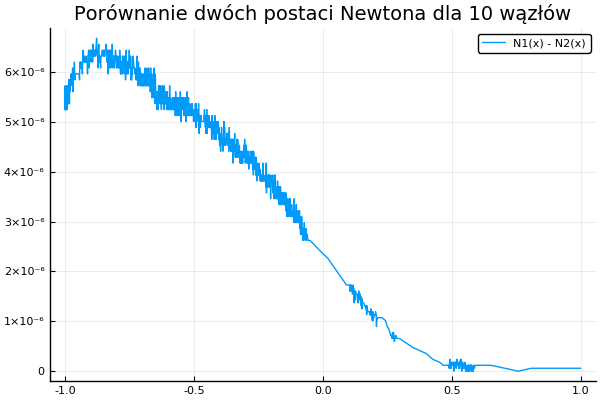
\includegraphics[scale=0.6]{NewtonsComp10.png}
  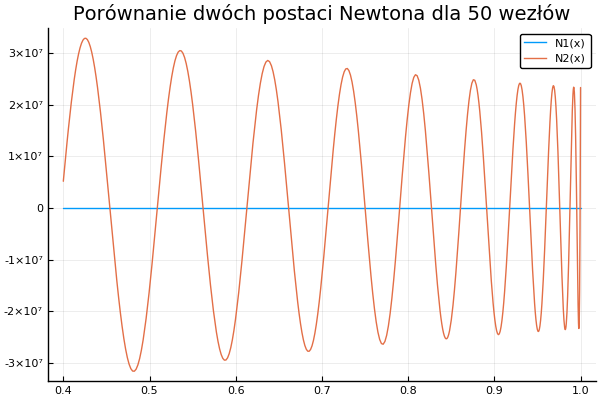
\includegraphics[scale=0.6]{NewtonsComp50.png}
\end{figure}

\newpage
\section{Porównanie postaci Lagrange'a i Newtona}
Porównanie metody Lagrange'a i Newtona zrobię na dwa sposoby:

\textbf{Sposób I:} Dla różnej ilości węzłów liczę wartość funkcji w jednym punkcie
, w którym wartość funkcji można łatwo policzyć i porównywać wyniki do wyniku 
dokładnego.

\textbf{Sposób II:} Dla różnej ilości węzłów liczę średni błąd w przybliżeniu 
funkcji wielomianem. (w tym przypadku ograniczyłem się jedynie do środka 
przedziału w którym interpolowałem, ponieważ na brzegach wielomiany \"wybuchają\"
co mocno psuje wyniki i utrudnia ich interpretację)

Każdym ze sposobów przeprowadzę testy na każdej z funkcji $f1(x) = \frac{1}{1+25x^2}$ i 
$f_2(x) = \arctan{x}$ z treści zadania oraz na $f(x) = \frac{\sin{x} + \cos{x} - 1}{x}$ z artykułu.
W tym sprawozdaniu pokażę, tylko po jednej z serii wyników dla jednego sposobu. 
Resztę wyników można uzyskać uruchamiając program załączony do sprawozdania.

Podczas prezentacji wyników będę używał oznaczeń:
\begin{itemize}
  \item L - postać Lagrange'a wyliczona normalnie
  \item LB - postać barycentryczna Lagrange'a
  \item N - postać Newtona
\end{itemize}

\subsection{Testy sposobem I}
W tabeli 1 i 2 przedstawione są wyniki testów policzone sposobem I dla funkcji 
$f(x) = \frac{1}{1+25x^2}$. Wartości wielomianów są liczone w punkcie $x=0$ gdzie funkcja $f(x)$
przyjmuje wartość 1. Do przybliżania funkcji użyłem parzystej liczby węzłów, aby żaden węzeł 
wielomianu nie trafił w funkcję w punkcie $x=0$ (wtedy postać barycentryczna daje dokładny wynik, 
natomiast inne postacie dają wynik dokładniejszy niż gdy węzłów jest tyle sam, ale żaden nie trafia
w punkt w którym liczymy wartość funkcji)

Porównując wyniki można zauważyć, że w tym przypadku metoda Newtona i Lagrange'a barycentryczna są
porównywalne. Zwykła postać Lagrange'a do pewnego czasu również jest z nimi porównywalna, jednak
dużo szybciej przestaje dawać wiarygodne wyniki (licząc w pojedynczej precyzji błąd bardzo 
gwałtownie).

\begin{table}[!h]
  \begin{minipage}{.55\linewidth}
    \begin{tabular}{c|ccc}
      \multicolumn{4}{c}{Pojedyncza precyzja}\\
      \hline \hline
      węzły & L & LB & N \\
      \hline
4 & 7.0701e-01 & 7.0701e-01 & 7.0701e-01\\
8 & 2.4736e-01 & 2.4736e-01 & 2.4736e-01\\
12 & 7.7033e-02 & 7.7035e-02 & 7.7035e-02\\
16 & 2.3784e-02 & 2.3754e-02 & 2.3753e-02\\
20 & 7.6084e-03 & 7.3214e-03 & 7.3186e-03\\
24 & 1.9788e-03 & 2.2569e-03 & 2.2549e-03\\
28 & 7.0565e-03 & 7.0584e-04 & 6.9487e-04\\
32 & -2.8920e-04 & 2.0075e-04 & 2.1392e-04\\
36 & -8.5097e-01 & 0.0000e+00 & 6.6161e-05\\
40 & -2.5313e+00 & -2.1219e-05 & 2.0742e-05\\
44 & -2.2632e+01 & 1.6093e-06 & 6.2585e-06\\
    \end{tabular}
  \end{minipage}%
  \begin{minipage}{.55\linewidth}
    \begin{tabular}{c|ccc}
      \multicolumn{4}{c}{Podwójna precyzja}\\
      \hline \hline
      węzły & L & LB & N \\
      \hline
4 & 7.0701e-01 & 7.0701e-01 & 7.0701e-01\\
8 & 2.4736e-01 & 2.4736e-01 & 2.4736e-01\\
12 & 7.7035e-02 & 7.7035e-02 & 7.7035e-02\\
16 & 2.3753e-02 & 2.3753e-02 & 2.3753e-02\\
20 & 7.3187e-03 & 7.3187e-03 & 7.3187e-03\\
24 & 2.2550e-03 & 2.2550e-03 & 2.2550e-03\\
28 & 6.9484e-04 & 6.9484e-04 & 6.9484e-04\\
32 & 2.1410e-04 & 2.1410e-04 & 2.1410e-04\\
36 & 6.5973e-05 & 6.5973e-05 & 6.5973e-05\\
40 & 2.0316e-05 & 2.0329e-05 & 2.0329e-05\\
44 & 6.2433e-06 & 6.2642e-06 & 6.2642e-06\\
    \end{tabular}
  \end{minipage}
  \caption{Testy dla funkcji $f(x) = \frac{1}{1+25x^2}$ w węzłach równoodległych}
\end{table}

\begin{table}[!h]
  \begin{minipage}{.55\linewidth}
    \begin{tabular}{c|ccc}
      \multicolumn{4}{c}{Pojedyncza precyzja}\\
      \hline \hline
      węzły & L & LB & N \\
      \hline
4 & 7.5030e-01 & 7.5030e-01 & 7.5030e-01\\
8 & 3.9174e-01 & 3.9174e-01 & 3.9174e-01\\
12 & 1.8277e-01 & 1.8276e-01 & 1.8276e-01\\
16 & 8.2953e-02 & 8.3096e-02 & 8.3107e-02\\
20 & 3.9197e-02 & 3.7643e-02 & 3.7590e-02\\
24 & 2.3706e-01 & 2.4916e-02 & 1.6984e-02\\
28 & 2.6273e+00 & -1.6117e-02 & 7.6719e-03\\
32 & -5.3937e+01 & -3.9829e-03 & 3.4652e-03\\
36 & 6.9465e+01 & -4.3844e-03 & 1.5634e-03\\
40 & 3.5042e+03 & -7.1418e-04 & 8.1325e-04\\
44 & -8.9059e+04 & 8.9669e-04 & -1.3804e-04\\
    \end{tabular}
  \end{minipage}%
  \begin{minipage}{.55\linewidth}
    \begin{tabular}{c|ccc}
      \multicolumn{4}{c}{Podwójna precyzja}\\
      \hline \hline
      węzły & L & LB & N \\
      \hline
4 & 7.5030e-01 & 7.5030e-01 & 7.5030e-01\\
8 & 3.9174e-01 & 3.9174e-01 & 3.9174e-01\\
12 & 1.8276e-01 & 1.8276e-01 & 1.8276e-01\\
16 & 8.3107e-02 & 8.3107e-02 & 8.3107e-02\\
20 & 3.7590e-02 & 3.7590e-02 & 3.7590e-02\\
24 & 1.6984e-02 & 1.6984e-02 & 1.6984e-02\\
28 & 7.6719e-03 & 7.6719e-03 & 7.6719e-03\\
32 & 3.4654e-03 & 3.4654e-03 & 3.4654e-03\\
36 & 1.5635e-03 & 1.5653e-03 & 1.5653e-03\\
40 & 7.5698e-04 & 7.0710e-04 & 7.0702e-04\\
44 & 3.7474e-04 & 3.1928e-04 & 3.1935e-04\\
    \end{tabular}
  \end{minipage}
  \caption{Testy dla funkcji $f(x) = \frac{1}{1+25x^2}$ w węzłach Chebysheva}
\end{table}
\subsection{Testy sposobem II}
W tabelach 3 i 4 przedstawione są wynikie testów policzone sposobem II dla funkcji 
$f(x) = \arctan{x}$. Dla 100 losowych punktów z przedziału $(-0.25, 0.25)$ liczę wartości 
funkcji oraz wilomianów oraz wyliczam średni błąd przybliżenia funkcji wielomianem. (Używam 
zawężonego przedziału, aby wartości, które znacznie odbiegają od wartości funkcji (blisko brzegów
przdziału) nie psuły nam wyników)

Analizując wyniki można zauważyć, że postac Newtona oraz postać Barycentryczna porównywalnie dobrze
przybliżają funkcję, z lekką przewagą postaci Barycentrycznej Lagrange'a. Drugą rzecza którą można
dostrzec jest to, że zwykła postać Lagrange'a na początku również całkiem dobrze przybliża naszą
funkcję.

\begin{table}[!h]
  \begin{minipage}{.55\linewidth}
    \begin{tabular}{c|ccc}
      \multicolumn{4}{c}{Pojedyncza precyzja}\\
      \hline \hline
      węzły & L & LB & N \\
      \hline
5 & 2.6829e-03 & 2.6829e-03 & 2.6829e-03\\
10 & 4.8759e-07 & 5.2956e-07 & 5.3035e-07\\
15 & 1.0801e-06 & 1.3479e-08 & 3.1562e-08\\
20 & 4.3028e-05 & 1.0231e-08 & 2.2703e-08\\
25 & 2.7507e-05 & 1.0959e-08 & 2.2862e-08\\
30 & 3.8815e-03 & 1.2892e-08 & 2.5083e-08\\
35 & 4.1679e-02 & 2.8662e-08 & 4.2219e-08\\
40 & 3.6640e-01 & 7.7431e-07 & 2.5700e-07\\
45 & 4.5399e+01 & 8.2285e-06 & 9.0291e-06\\
50 & 1.0111e+03 & 4.1527e-05 & 2.3304e-04\\
    \end{tabular}
  \end{minipage}%
  \begin{minipage}{.55\linewidth}
    \begin{tabular}{c|ccc}
      \multicolumn{4}{c}{Podwójna precyzja}\\
      \hline \hline
      węzły & L & LB & N \\
      \hline
5 & 2.6829e-03 & 2.6829e-03 & 2.6829e-03\\
10 & 5.3058e-07 & 5.3058e-07 & 5.3058e-07\\
15 & 1.2895e-08 & 1.2895e-08 & 1.2895e-08\\
20 & 3.9830e-12 & 4.0104e-12 & 4.0103e-12\\
25 & 5.7056e-13 & 9.5646e-14 & 9.5640e-14\\
30 & 1.8294e-11 & 3.4606e-17 & 5.1994e-17\\
35 & 2.8274e-10 & 2.4318e-17 & 3.6603e-17\\
40 & 2.1502e-09 & 2.9327e-17 & 3.8217e-17\\
45 & 1.4285e-07 & 2.7555e-17 & 4.6262e-17\\
50 & 1.1845e-06 & 3.0944e-17 & 4.8910e-17\\
    \end{tabular}
  \end{minipage}
  \caption{Testy dla funkcji $f(x) = \arctan{x}$ w węzłach równoodległych}
\end{table}

\begin{table}[!h]
  \begin{minipage}{.55\linewidth}
    \begin{tabular}{c|ccc}
      \multicolumn{4}{c}{Pojedyncza precyzja}\\
      \hline \hline
      węzły & L & LB & N \\
      \hline
5 & 3.3980e-03 & 3.3979e-03 & 3.3979e-03\\
10 & 1.8917e-06 & 1.9049e-06 & 1.9020e-06\\
15 & 2.9029e-05 & 2.0269e-07 & 1.9899e-07\\
20 & 2.2263e-04 & 1.0111e-08 & 1.8334e-08\\
25 & 6.8357e-02 & 2.0048e-07 & 1.9839e-08\\
30 & 3.2312e+00 & 6.0604e-05 & 6.8542e-08\\
35 & 1.5109e+02 & 6.4557e-05 & 9.2488e-06\\
40 & 3.3453e+03 & 9.9275e-05 & 2.5281e-03\\
45 & 8.9749e+05 & 2.4093e-02 & 9.0552e-02\\
50 & 6.8779e+07 & 1.5818e-01 & 4.4490e+00\\
    \end{tabular}
  \end{minipage}%
  \begin{minipage}{.55\linewidth}
    \begin{tabular}{c|ccc}
      \multicolumn{4}{c}{Podwójna precyzja}\\
      \hline \hline
      węzły & L & LB & N \\
      \hline
5 & 3.3979e-03 & 3.3979e-03 & 3.3979e-03\\
10 & 1.9029e-06 & 1.9029e-06 & 1.9029e-06\\
15 & 2.0145e-07 & 2.0145e-07 & 2.0145e-07\\
20 & 1.6768e-10 & 1.6776e-10 & 1.6776e-10\\
25 & 4.0374e-11 & 1.7993e-11 & 1.7993e-11\\
30 & 4.2430e-09 & 2.2047e-14 & 2.2048e-14\\
35 & 3.3488e-07 & 2.2782e-15 & 2.2771e-15\\
40 & 4.1313e-05 & 2.4281e-17 & 5.0537e-17\\
45 & 4.3644e-03 & 7.2035e-16 & 4.6979e-17\\
50 & 1.9391e-02 & 1.4790e-12 & 6.5638e-17\\
    \end{tabular}
  \end{minipage}
  \caption{Testy dla funkcji $f(x) = \arctan{x}$ w węzłach Chebysheva}
\end{table}

\section{Podsumowanie}
Po wykonaniu wszystkich testów mogę stwierdzić, że dla wszystkich stopni wielomianów, 
metoda barycentryczna jest porównywalna lub lepsza od metody Newtona. Im mniejszy jest 
stopień wielomianu, tym mniejsza różnica jest pomiędzy tymi dwoma postaciami.

Warto również zauważyć, że zwykła postać Lagrange'a dla małych stopni wielomianów równie dobrze 
przybliża funkcję jak postać barycentryczna i postać Newtona. Co prowadzi do wniosku, że gdy 
przybliżamy funkcję wielomianami niskiego stopnia, nie musimy konstruować bardziej skomplikowanych
(postaci wielomianu interpolacyjnego. 

Zamiana jednej postaci na drugą według algorytmu podanego w tym sprawozdaniu może być wykorzystywana, 
jeśli stopień wielomianu nie jest duży. Jedynym powodem, dla którego można to zrobić jest chęć 
wielokrotnego liczenia wartości wielomianu, gdyż złożoność obliczania wartości w punkicie dla postaci
Newtona jest lepsza ($O(n)$ zamiast $O(n^2)$).

\begin{thebibliography}{9}
  \bibitem{werner}
  W. Werner, 
  \textit{Polynomial interpolation: Lagrange versus Newton}, 
  Math. Comp., 43 (1984), pp. 205-217.

  \bibitem{bli}
    Jean-Paul Berrut, Lloyd N. Trefethen,
    \textit{Barycentric Lagrange interpolation}
    SIAM Review Vol. 46, No. 3, pp. 501–517.
\end{thebibliography}
\end{document}
